\documentclass{standalone}
\usepackage{tikz}
\usetikzlibrary{decorations.pathreplacing}
\usepackage{amsfonts}


\begin{document}
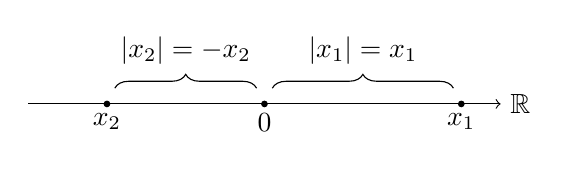
\begin{tikzpicture}
% Draw the real line
  \draw[->] (-3,0) -- (3,0) node[right] {$\mathbb{R}$};
  
  % Draw the point 'x' and '0'
  \filldraw (0,0) circle (1pt) node[below] {0};
  \filldraw (2.5,0) circle (1pt) node[below] {$x_1$};
  \filldraw (-2,0) circle (1pt) node[below] {$x_2$};
  
  % Draw the brace and label it
  \draw[decorate,decoration={brace,amplitude=5pt}] (0.1,0.2) -- (2.4,0.2) node[midway,above=5pt] {$|x_1|=x_1$};
  
  \draw[decorate,decoration={brace,amplitude=5pt}] (-1.9,0.2) -- (-0.1,0.2) node[midway,above=5pt] {$|x_2|=-x_2$};
  
  
  
  \end{tikzpicture}
\end{document}